\documentclass[8pt]{extarticle}
\usepackage{multicol}
\usepackage[margin=0.3in]{geometry}
\usepackage{paralist}
\usepackage{parskip}
\usepackage{amsmath}
\usepackage{float}
\usepackage{graphicx}
\usepackage{natbib}

\begin{document}
\begin{multicols}{2}
\section{Introduction to CV \& Paradigms}
Computer vision is going from an image to understanding what's in an image.

\subsection{Introduction}
\subsubsection{Visual Shortcuts}
\begin{compactitem}
    \item Light comes from above
    \item Objects have largely convex borders
    \item Lines are expected to be continuous
    \item Objects are normally not viewed from below
    \item Faces are upright
\end{compactitem}

\subsubsection{Gesalt principles}
\begin{compactitem}
    \item Proximity - How class things are to each other
    \item Similarity - How similar things look to each other
    \item Closure - Automatically complete broken lines
    \item Common Fate - Perception of the path a object follows through space
\end{compactitem}

\subsubsection{Human Vision is:}
\begin{compactitem}
    \item stereo - binocular vision
    \item foveal - 100\% visual acuity (direct line-of-sight accuracy)
    \item attentive - Focuses on points of interest
    \item integrated - What you perceive is coloured by what you've seen before \& what you expect
\end{compactitem}


\subsection{Paradigms}
\subsubsection{Marr's/Reconstructionist}
\begin{compactitem}
    \item Image - 2D lattice of light information.
    \item Raw Primal Sketch - Locations of (sudden) changes in intensity. This represents structure.
    \item Full Primal Sketch - Identified locations are grouped into contours \& boundaries
    \item 2 1/2D Sketch - Going from images to surfaces (Shape from X). Local relative depth \& surface orientation.
    \item 3D Model - High level 3D description of the world. Generalised cylinders, symbolicl representation...
\end{compactitem}

\subsubsection{Qualitative Vision}
\begin{compactitem}
    \item Sensors are noisy. Difficult to extract precise information.
    \item Often it is only necessary to know the relations between objects.
    \item Goes from ``pixels to predicates''.
\end{compactitem}

\subsubsection{Active Vision}
\begin{compactitem}
    \item Moving the camera to improve perception
    \item Disambiguates \& solves singularities. Solves occlusions
    \item Popular in robotics (SLAM - Simultaneous Localisation And Mapping)
\end{compactitem}

\subsubsection{Vision through ML}
\begin{compactitem}
    \item Relies on datasets with large variation to train systems that work with a large variation of input images.
    \item Follows a sort of TDD approach. Must have reliable results for a system to be worth anything.
\end{compactitem}


\section{Image Formulation}

\subsection{General}
\begin{compactitem}
    \item Objects projected onto an image plane through a pinhole camera.
    \item Larger objects appear closer.
    \item Issue: ``Father Ted Problem'' - Camera-Object distance is not recoverable from a single viewpoint.
\end{compactitem}

\subsection{Radiosity}
\begin{compactitem}
    \item Brightness depends on: light arriving \& leaving surface, relative position of the light source and viewer, and the nature of the surface.
    \item Lambertian: Matte reflection. Brightness only depends on the angle between light and surface normal.
    \item Specular: Shiny. Light leaves along the same vector reflected about the surface normal.
\end{compactitem}

\subsection{Digitizing}
\begin{compactitem}
    \item Images are not continuous. Leads to limited resolution.
    \item Pixel values are not continuous either. Limited number of discrete possible choices. (Greyscale \& Colour)
    \item Colour Spaces
    \begin{compactitem}
        \item Red Green Blue (RGB): 256 colours between 0-255.
        \item Hue Value Saturation (HSV): Hue - represents colours, Saturation - quantity of colour, Value - Dark to light scale.
        \item CIE L*a*b: better separation of luminance from colour.
    \end{compactitem}
\end{compactitem}

\section{Edge Detection, Grouping \& Features}

\subsection{Edges}
\begin{compactitem}
    \item Parts of images are perceived as regions of interest. These are surrounded by boundaries, which are made of edge pixels.
    \item Intensity profile: signal changes sharply at the edges of of an object in the scene. The sharper the change, the more clearer the boundary.
    \item Locating intensity changes: Differentiate it and look for extrema values.
\end{compactitem}

\subsubsection{Detecting changes in intensity}
\textbf{Sobel Edge detector}: Differentiate the image profile by convolving an image mask (kernel). Typically we use a 3x3 mask to give a local averaging effect to reduce noise, and use both a horizontal and vertical kernel to look for horizontal and vertical edges. The computed horizontal and vertical components are combined using the RMS formula $S(x) = \sqrt{S_h(x) + S_v(x)}$ to produce an array of \textbf{edge strengths}. Predominant direction can be deduced by inverse tangent $\theta(x) = tan^{-1}(S_h(x) / S_v(x))$. Issues: \textit{Thickening} and choice of \textit{threshold}.

\textbf{Laplacian Of Gaussians}: Computation of the second derivative gives a sharp up-down response the crosses zero at the edge. To get directionality, the two         differentials are merged using the laplacian.
    \begin{equation}
        \nabla^2I(x,y) = \frac{\partial^2 I(x,y)}{\partial x^2} + \frac{\partial^2 I(x,y)}{\partial y^2}
    \end{equation}
    To reduce the noise of the second derivative we can blur the image with a Gaussian function, smoothing the resulting 2nd order derivatives. We must choose the $\sigma$ parameter for blurring. Process for LoG edge detector: choose small $\sigma$, blur image, filter with laplacian (zeros are edges), increase sigma \& repeat. This accumulates a pyramid of edge detections.

\textbf{Canny Edge Detector}: Key points:
    \begin{compactitem}
        \item Uses first order derivatives.
        \item Iterated Gaussian blur.
        \item Non-maximal suppression. Suppress effects of thickening.
        \item Supports tracking (hyterisis) to link weak evidence to strong.
    \end{compactitem}

\subsection{Grouping Edges}
Edge detection only extracts single or small groups of pixels. We need higher level features (straight lines, curves, geometric shapes). The approach to grouping can either be top down or bottom up.

\begin{compactitem}
    \item \textbf{Bottom up}: Pixels are grouped by edge following. Move from one edge pixel along direction until you find the next. Issues: camera \& digitisation noise, gaps, complex topology, starting point dependancy, and multiple paths.

    \item \textbf{Top down}: Model what is sought and projectit onto the image. Issues: We need to choose a model, how to project, noise, matching complexity.
\end{compactitem}

\subsubsection{Approaches}

\textbf{Hough Transform}: All lines going through a pixel create a curve in \textit{line space} (rho, theta space) of the line parameters, painted in an accumulator array. Voting from all edge pixels. High values in accumulator indicate lines (use threshold). Same principle can be used with other geometric shapes. For practical reasons the equation of a line used is defined by $x cos(\theta) + y sin(\theta) + r = 0$.\\

\begin{figure}[H]
    \centering
    \includegraphics[width=0.4\textwidth]{Hough_transform_diagram.png}
    \caption{Diagram showing the parameterised lines used in the hough transform.}
    \label{fig:hough-transform}
\end{figure}

Pros:
\begin{compactitem}
    \item Good solution to geometrical feature matching
    \item Can group wildly separated pixels.
\end{compactitem}
Cons:
\begin{compactitem}
    \item Can group wildly separated pixels.
    \item Depends on a number of parameters (grids size (think quantisation), threshold).
    \item Needs enough evidence to work.
\end{compactitem}

\textbf{RANSAC}: RANdom SAmpling with Consensus. Fit model to a random subset of points (sample), build a consensus set (other points that fit the model), evaluate quality of the model though the total error of the consensus set, repeat many times. Number of iterations required can be based on the probability of outliers, acceptable error, and size of sample set. Good technique for modelling data which is likely to be heavily effected by outliers. Can be used with a more general model than just simple lines.

\subsection{Features}
A feature is a higher level element in a scene. Many things can be features such as textures, corners, ellipses, projects or rectangles, ribbons etc. What makes a good features?
\begin{compactitem}
    \item Repeatability: Can we find the feature again in?
    \item Distinctiveness: is it different from the rest of the image, or distinctive in terms of its \& the image's statistics?
    \item Locality: Features should be local, i.e not the entire image!
    \item Easy to find: Are there enough of them to use for matching (quantity)?
    \item Accuracy: do they pinpoint a thing with precision?
    \item Efficiency: an we compute them quickly?
\end{compactitem}

\subsubsection{Techniques}
If we wish to find something in an image, then find it again in another we need something common feature that is easy to locate again. Corners are good because \textit{1)} they reside on an edge where there is a change in intensity, \textit{2)} A corner is a place where edges meet. Corners can be found quickly becuase they are very distinctive, the local neighbourhood is usually quite unique.
\\ \\
\textbf{Harris Corners}: Don't just look at a patch for matching, look around the neighbourhood of the patch. Follows the equation:
\begin{equation}
    E(u,v) = \sum\limits_{x,y} w(x,y)[I(x+u, y+v) - I(x,y)]^2
\end{equation}
where $w$ is the window function, $I$ is the image intensity $u,v$ are parameters to shift the image slightly. The window can either be a hard threshold (0 or 1) if the image is in the window or not, or it can be a Gaussian. If Gaussian then differences in intensity near the middle of the window count for more. Having defined a cost function $E(u,v)$ we maximise it to detect corners.

\textbf{KLT Corners}: Kanade-Lucas-Tomasi. Similar to Harris. Main difference is the scoring function. KLT tends to find less points of interest when compared to Harris.
\\ \\
\textbf{SIFT}: Scale Invariant Feature Transform. A technique that produces features which are:
\begin{compactitem}
    \item Invariant to scale
    \item Invariant to rotation in the image plane
    \item Invariant to small rotations in depth/translations
    \item Contain a local description of the image
\end{compactitem}

SIFT achieves scale invariance by using a difference of Gaussians (DoG) of successive images Doesn't use LoG because it's expensive. The extrema of the DoG in space \& scale give scale invariance. Features are selected if they have good enough contrast, i.e. they're on a corner (peak of a DoG). Sub-pixel localisation is handled by locally fitting a quadratic model to DoG. Method is protected by a patent.
\begin{itemize}
    \item \textbf{Orientation Invariance}: Image gradient computed around each feature's scale. Orientation histogram is created for each feature to represent a Gaussian weighted orientations. Features are then created for each major orientation.
    \item \textbf{Feature Description}: Image gradient invariant to changes in illumination and contrast (after normalisation). Local gradients grouped around features in normalised histograms.Grouping gives some invariance to small geometrical transformations.
\end{itemize}

\textbf{Scale Space} As the scale of the image increases, the number of zero crossings decreases because the signal gets smoother. This can be converted to a interval tree of a which scale the zero crossing breaks down into other crossings. Scale is the sigma value of a Gaussian. SIFT filters images with Gaussians at different widths. Finding the extrema of the DoG gives us points of interest.

We can match keypoints between two scenes by using nearest neighbour matching. We can use the ratio of the distance between the 1st and 2nd nearest neighbour. If the ratio is small then there is ambiguity, if large, first match is good.

\textbf{SURF}: Speeded Up Robust Features. Uses lots of small tricks to improve the performance of SURF. For example it uses box features instead of LoG features which are quicker to compute. This is known as the difference of boxes, the integral image representation can be used to make computation quicker.

\subsection{Appearance \& Comparing Images}
Comparing images generally follows a process similar to convolution. Notations used in this section:
\begin{compactitem}
    \item $I$: image
    \item $A$: appearance (image) of the object
\end{compactitem}
$A$ is smaller than $I$. Origin of images in top left corner.
\\ \\
\textbf{Euclidean Distance}
The sum of squared differences is the same but without the square root. Simple, but not normalised.
\begin{equation}
    d(x,y) = \sqrt{\sum\limits_{i}\sum\limits_{j} (I(x,y) - A(x,y))^2}
\end{equation}
\\ \\
\textbf{Correlations}:
Correlations are independent of the brightness of images and it gives a small amount of robustness to noise and partial matches. A threshold may also be used. However it is not as quick as Euclidean distances and not prefect. Can compute correlation coefficients between -1 and 1. Where high is a very positive match and low is a very negative match.

\section{Motion}
Used to detect interesting things in videos. Quite often the things of interest will be moving. Two ways of approaching motion: Find things that aren't moving and ignore them (background subtraction), try and capture motion directly (optical flow).

\subsection{Background subtraction}
Key points:
\begin{compactitem}
    \item requires a static camera!
    \item assumes scene is still
    \item assumes lighting doesn't change much
    \item assumes time series doesn't have ``flicker''
\end{compactitem}

When an object passes in front of a camera there is going to be a change in the intensities within the image which can be seen in each frame over time. However, the camera is affected by noise from the sensor and also from lighting within the scene not being perfectly constant. Lighting in particular leads to the problem of drift. This leads use to  use a moving average which is robust to small variations corresponding to noise. It can deal with:

\begin{compactitem}
    \item lighting changes
    \item objects put down in the scene
    \item circumstances where the scene isn't empty to begin with.
\end{compactitem}

Equation for moving background subtraction is:
\begin{gather}
    \|I_n - B_{n-1}\| < T \implies background \\
    \|I_n - B_{n-1}\| > T \implies foreground
\end{gather}
where:
\begin{equation}
    B_{n-1} = \frac{1}{w}\sum\limits_{j=(n-w)}^{n-1}I_j
\end{equation}

However, this does not deal with the issue of flicker very well. To solve flicker, more complicated models can be used. E.g. Explicitly modelling the noise process, treating each pixel as a time series, or a post-processing step. Complications:

\begin{compactitem}
    \item It's actually 3D. We've been treating each pixel individually, but they often vary together (RGB space).
    \item Variation is not constant. Some objects or noise will vary more than others. Simple threshold means you can't take this into account. Noise is often Gaussian, so model it as such.
    \item We need to think about the background at one place being more than one colour. In a Gaussian context this means that it is sampled from more than one distribution a.k.a Expectation Maximisation.
\end{compactitem}

\textbf{Solution}: Model noise as a Gaussian. Use a threshold based on the width of a Gaussian. Pixels with a lot of noise have a higher threshold. This leads to \textbf{Gaussian Mixture Modelling}

\begin{compactitem}
    \item Deals with complicated background
    \item Robust to noise
    \item Can handle shadows OK. (can even detect shadows)
\end{compactitem}

\subsection{Optical Flow}
\textbf{Montion Field}: projection of the motion of objects in the world onto the image plane. \\ \\
\textbf{Optical Flow}: apparent motion of brightness patterns on the image. An approximation of the motion field. Issues:
\begin{compactitem}
    \item aperture problem - ambiguities; Homogeneous sphere rotating seems static, static homogeneous sphere with rotating light source appears to move. ``Barber's Pole'' illusion.
    \item apparent motion
\end{compactitem}

\subsubsection{Dense Optical Flow}
Appearance based method. Uses correlation coefficients (or similar) n small image patches around each pixel. Uses a differential method. Assume near by points in the image have similar brightness, find nearby points that satisfy this, work out direction for travel. Leads to the following optical flow constraint:

\begin{equation}
    u\frac{\partial I}{\partial x} + v\frac{\partial I}{\partial y} + \frac{\partial I}{\partial t} = 0
\end{equation}

This equation has a infinite number of solutions. There are issues relating to:
\begin{compactitem}
    \item Noise
    \item assumes there is only one motion (rigidity assumption)
    \item assumes there are no discontinuities in motion (smoothness).
\end{compactitem}

Solutions are found by minimising the smoothness and optical flow constraint equations. Computing the gradient requires lots of features in all directions. Assumed smoothness between features can help interpolate missing values.

\subsection{Sparse Optical Flow}
A.k.a Feature tracking. Basic principle: We have a feature that we should be able to find again in one frame, then we find the one which looks most like it in the next frame.

\begin{compactitem}
    \item If there's not match above a quality threshold then delete it
    \item If there's a match then the displacement vector between them is the motion vector
\end{compactitem}

Further speed ups are possible using assumptions. We can assume that things don't move too fast (constrain the search to a window around feature). We can assume that things move in a fairly coherent way (contrain search in direction of motion).

Pros of technique:
\begin{compactitem}
    \item You can track still things.
    \item It's fast
    \item It's robust
\end{compactitem}

Cons:
\begin{compactitem}
    \item You can track still things.
    \item Tracks can get lost. (screen edge, occlusions)
    \item You need to decide when to reinitialise
\end{compactitem}

\subsection{Tracking}
Use to draw conclusions over a series of frames. General framework for tracking: the update-predict-measure cycle. We have an idea about what will change, we make a prediction, then we measure and update our model accordingly.

Pros of tracking:
\begin{compactitem}
    \item Smooths data - update your estimate of location based on the prediction and the measurement.
    \item Constrains search - You start looking for your target in the location of the prediction.
\end{compactitem}

Issues with tracking:
\begin{compactitem}
    \item Initialisation - What to choose to track.
    \item Having more than one thing to track
    \item Losing target due to motion/occlusion. Trackers may also ``drift'' off target.
    \item Losing target due to appearance change. Sometimes the thing we're tracking changes a lot.
\end{compactitem}

A Kalman filter is an example of a system for tracking things over multiple frames.
\begin{figure}[H]
    \centering
    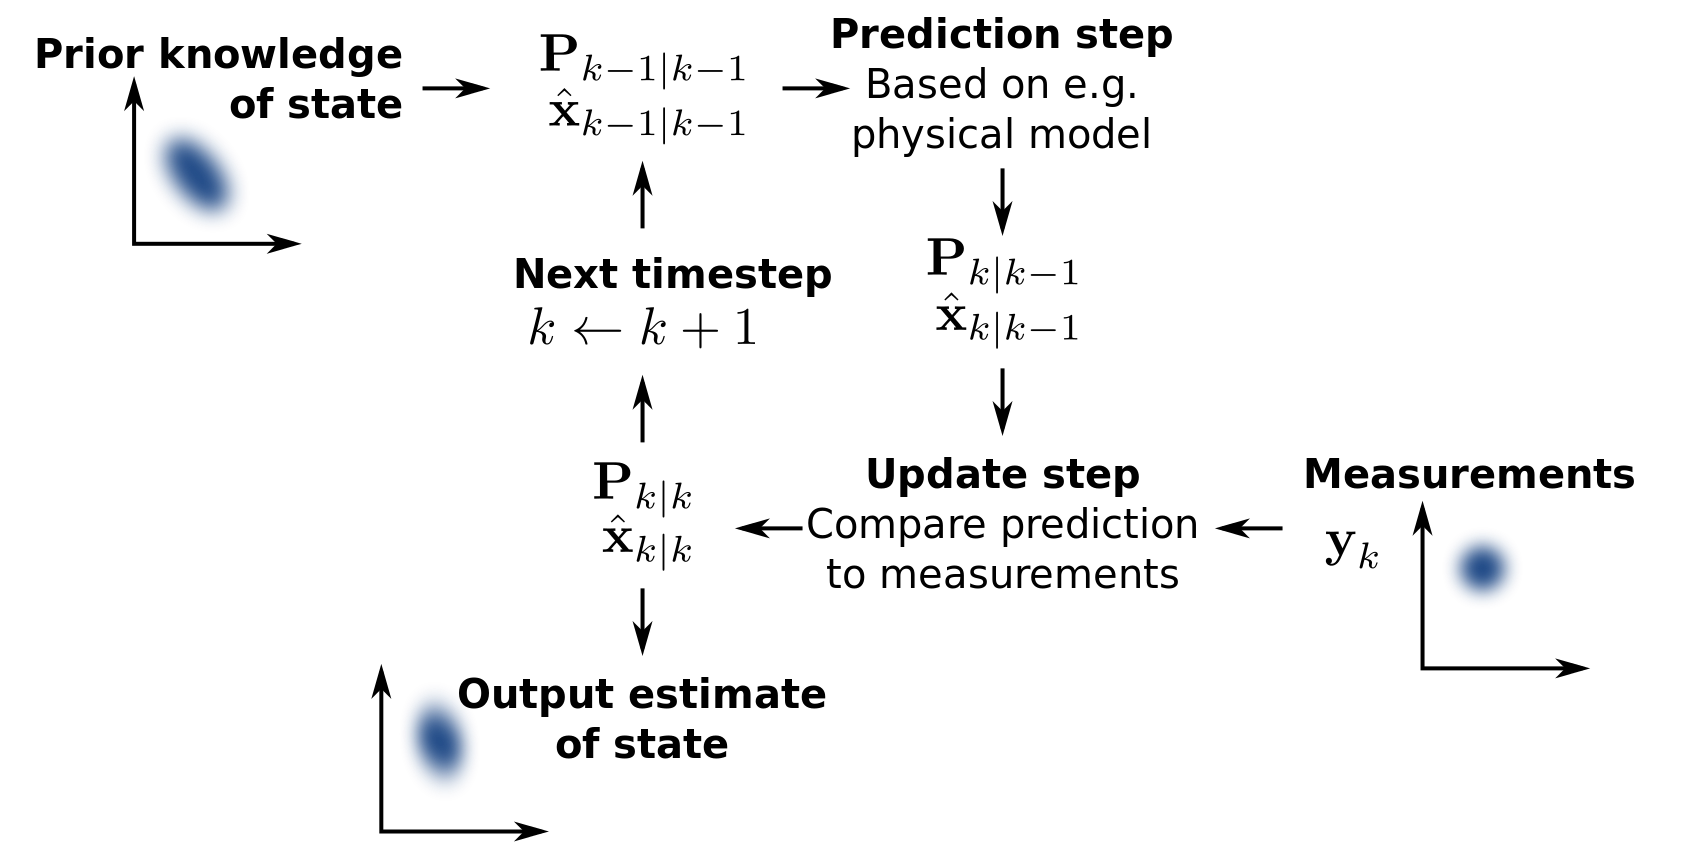
\includegraphics[width=0.4\textwidth]{Kalman_filter.png}
    \caption{Basic process of a Kalman filter}
    \label{fig:kalman-filter}
\end{figure}

\section{Objects}
Objects are higher level concepts within a scene. They are many and varied.

\begin{compactitem}
    \item Detection: Taking lots of examples of an object and trying to find what's common. Modelling \textit{within class} variation
    \item Recognition: Finding a single specific object from a concept. Modelling \textit{between class} variation
\end{compactitem}

General framework for object detection
\begin{enumerate}
    \item Look at lots of examples of your object (with high variation)
    \item Represent them in some way (this is a model).
    \item Take the object you wish to find and represent it in some way. (this is your model).
    \item Try to find matches between the model and the image.
\end{enumerate}

What data is available or will be captured?
\begin{compactitem}
\item 2D vs. 3D
\item range of viewing conditions
\item available context
\item segmentation cues
\end{compactitem}

How can we represent the object of interest?
\begin{compactitem}
\item local 2D features
\item 3D surfaces images
\end{compactitem}

How many objects are involved in a single image or data set?
\begin{compactitem}
\item small: brute force search
\item large: ??
\end{compactitem}

Questions about the representation. These are related to what makes a good feature.
\begin{compactitem}
    \item Accessibility: can the representation be computed from the image using reasonable resources?
    \item Scope: can the scheme represent a sufficient variety of shapes?
    \item Uniqueness: do two identical shapes have the same representation?
    \item Stability: do two similar shapes have close representations?
    \item Sensitivity: do two slightly different shapes differ in their representations?
\end{compactitem}

Key elements of object detection
\begin{compactitem}
    \item Training set
    \item Representation (choice of feature type)
    \item Model learning (or calculation)
    \item Representation of test images
    \item Matching of model to test images
\end{compactitem}

Once you have a reliable feature detector (e.g. SIFT or SURF) you can built on this to find specific or general objects. Either you look for specific combinations of features or you try to generalise your features to deal with variation (as in Viola-Jones).

Feature detectors have a bit of invariance built in. SIFT and SURF can deal with rotation and scale and a bit of out of plane rotation. Technically these are affine transformations.

\subsection{Recognising Objects}
Select the object you're interested in a find points of interest. Each feature is a representation of a small part of the image.

\textbf{Homography}: The same scene viewed from different perspectives results in two image planes. The transformation of points from one image plane to another is called a homography. Obviously the points are noisy, but we can fit them with something like RANSAC. If we can fit a plane to the image that matches well with the test image then we've found our match. Issues: not good with multiple classes, what about all sorts of orientations?

\textbf{Modelling variation in classes}: e.g. Bag-of-words; not structure, no order, just features in a bag. Key points about bag-of-words:
\begin{compactitem}
    \item It needs a training set of labelled objects
    \item It uses clustering to turn features into visual words
    \item It makes no assumption about the spatial relationships between these
    \item If a cow is standing on its head, it’ll get detected As will a pile of cow parts (ew).
    \item This gives it a lot of robustness to variation, but can have some (obvious) side effects
\end{compactitem}

Other approaches: use parts or structure models. 3D structure models (particularly for pose estimation). These often have a simialr representation, but use different matching strategies which enforce spatial organisation.

\section{Shape From X}
Moving beyond detection and localisation in the x,y plane. Interested in recovering the 3D structure of objects and scenes.
\begin{figure}[H]
    \centering
    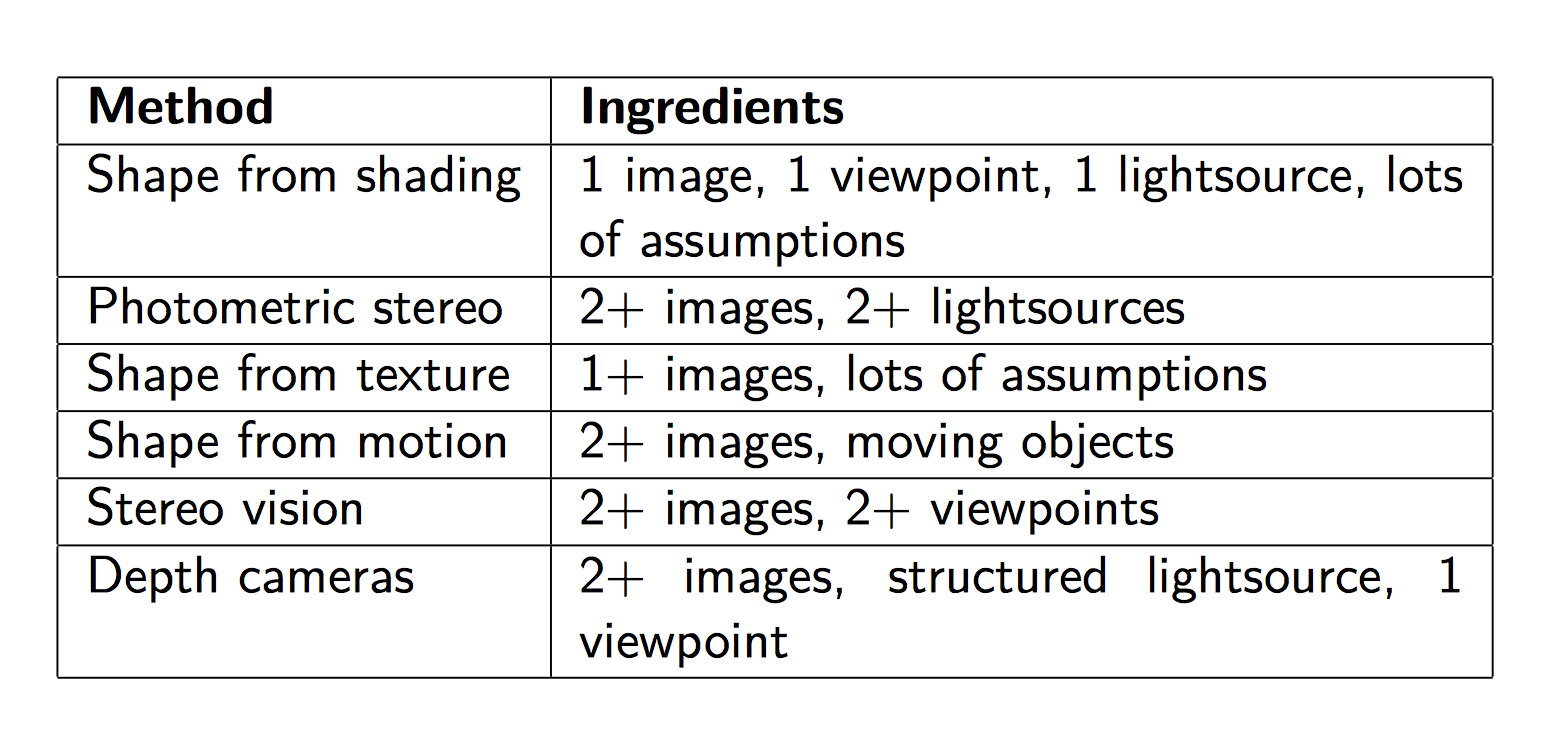
\includegraphics[width=0.4\textwidth]{2dto3d.png}
    \caption{Table comparing 2D to 3D techniques.}
    \label{fig:2D-to-3D}
\end{figure}

\subsection{Shape From Shading}
Brightness can be used to recover some 3D information about the world. Brightness of a point in the world depends on:
\begin{compactitem}
    \item where the light source(s) is (are)
    \item where the viewer is
    \item local orientation of the surface properties of the surface
\end{compactitem}
However, there are ambiguities such as the hollow face illusion.

\textbf{Bidirectional Reflectance Distribution Function}: a.k.a BDRF. Fraction of the incident light reflected in the direction of the viewer. Depends upon the angles of incidence and emittance and the phase angle. Largely a property of the surface. Defines how light interacts with the surface. Difficult to establish in even the most simple cases. Often determined experimentally: take lots of photos under known lighting conditions. Often assume single, simple light source, no reflections.

We're trying to extract 3D information about a scene. Surface orientation can be described by a normal. Normals are unit vectors so they only encode direction. We can describe these with two quantities:

\begin{gather}
    p = \frac{\partial z}{\partial x}, q = \frac{\partial z}{\partial x}
\end{gather}

These define the gradient space $(p,q)$. Parallel planes all map to a single point. Perpendicular plane maps to a point at the origin. Moving off the origin corresponds to tilting and slanting the surface.

\textbf{Reflectance Map}: Can be computed from the BDRF for a surface as a function of surface orientation in gradient space. Using this a single intensity gives us a possibl set of orientations. Global solution found by integration of gradient and image space together. Issues: Smoothness assumption!

Shape from shading gives us an estimate of reflectance but it comes at the price of assumptions. We can reduce the assumptions by using multiple lighting conditions. Multiple lights remove ambiguities about the surface. Issues: assumes the scene does not move. To calibrate: illuminate the scene with one light at a time take photo of sphere with similar reflectance to object you're imaging. Then image the object and use the calibrated sphere images to reconstruct surface geometry.

\subsection{Shape From Texture}
Images depict a regularly occurring event. \textit{Isotropic}: rotation perpendicular to the plane does not change the texture. \textit{Homogeneous}: texture looks the same everywhere. \textit{Texel}: Basic texture element the repetition of which creates the texture.

Textures can be represented in a variety of ways such as:
\begin{compactitem}
    \item Explicit Texel estimation/detection
    \item Filter response
    \item Statistical methods
\end{compactitem}

For textures which are planes they may be characterised by their tilt and slant. If isotropic the texture is recovered through a project (the projection isn't isotropic). If homogenous then the gradient is used (changes in density indicates shape). The global case typically use local methods and then interpolated. Issues: Assumes homogenity and smoothness.

\subsection{Shape From Motion}
Incremental reconstruction of shape as a set of distances between points. The initial structure is assumed to be flat, therefore giving initial distances between points. For each new image update the distances so as to minimise the distance between points while taking into account the new values. Issues: Rigidity assumption and parallel projection. (Some non-rigidity may be handled).

\subsection{Shape From Occlusions}
Produces contours due to a discontinuity in depth. Often corresponds to silhouette of object. Smoothness both within the contour but also along. Several images may also be used. Projection of generalised cone containing object, the intersection of cones is the object. Issues: assumes each point on a contour corresponds to a point on the object. Nearby contour points correspond to nearby object points, points on contour correspond to planar points on the object.

\subsection{Shape From Focal Length}
Choose a lens with a narrow depth field and vary the focus which gives depth. Can be done with specalist cameras and via ad-hoc methods.

\section{Stereo Vision}
Getting 3D information about a scene from two or more 2D images. Prequisites for 3D reconstruction :

\begin{compactitem}
    \item Perfect Cameras - we have cameras that a very good.
    \item Geometry of the system - measured but we can do it.
    \item Finding correspondences - hard.
\end{compactitem}

\textbf{Correspondace problem}: Finding corresponding points in two different images. Problem is which areas should be matched. Approaches can be area/appearence, feature or motion flow based.

\textbf{Disparity Map}: Horizontal/vertical displacement between corresponding pixels. The result of the correspondence process. Closely related to scene depth.

Matching issues:
\begin{compactitem}
    \item Camera-related problems
    \item Scene and/or images related problems
    \item Viewpoint-related problems
    \item Illumination conditions
    \item Specular Reflections
    \item Lack of texture
    \item Occlusions
    \item Ambiguity
    \item Multiple interpretations
\end{compactitem}

Using epipolar geometry we can restrict the position of the corresponding pixel in a second image.
\begin{figure}[H]
    \centering
    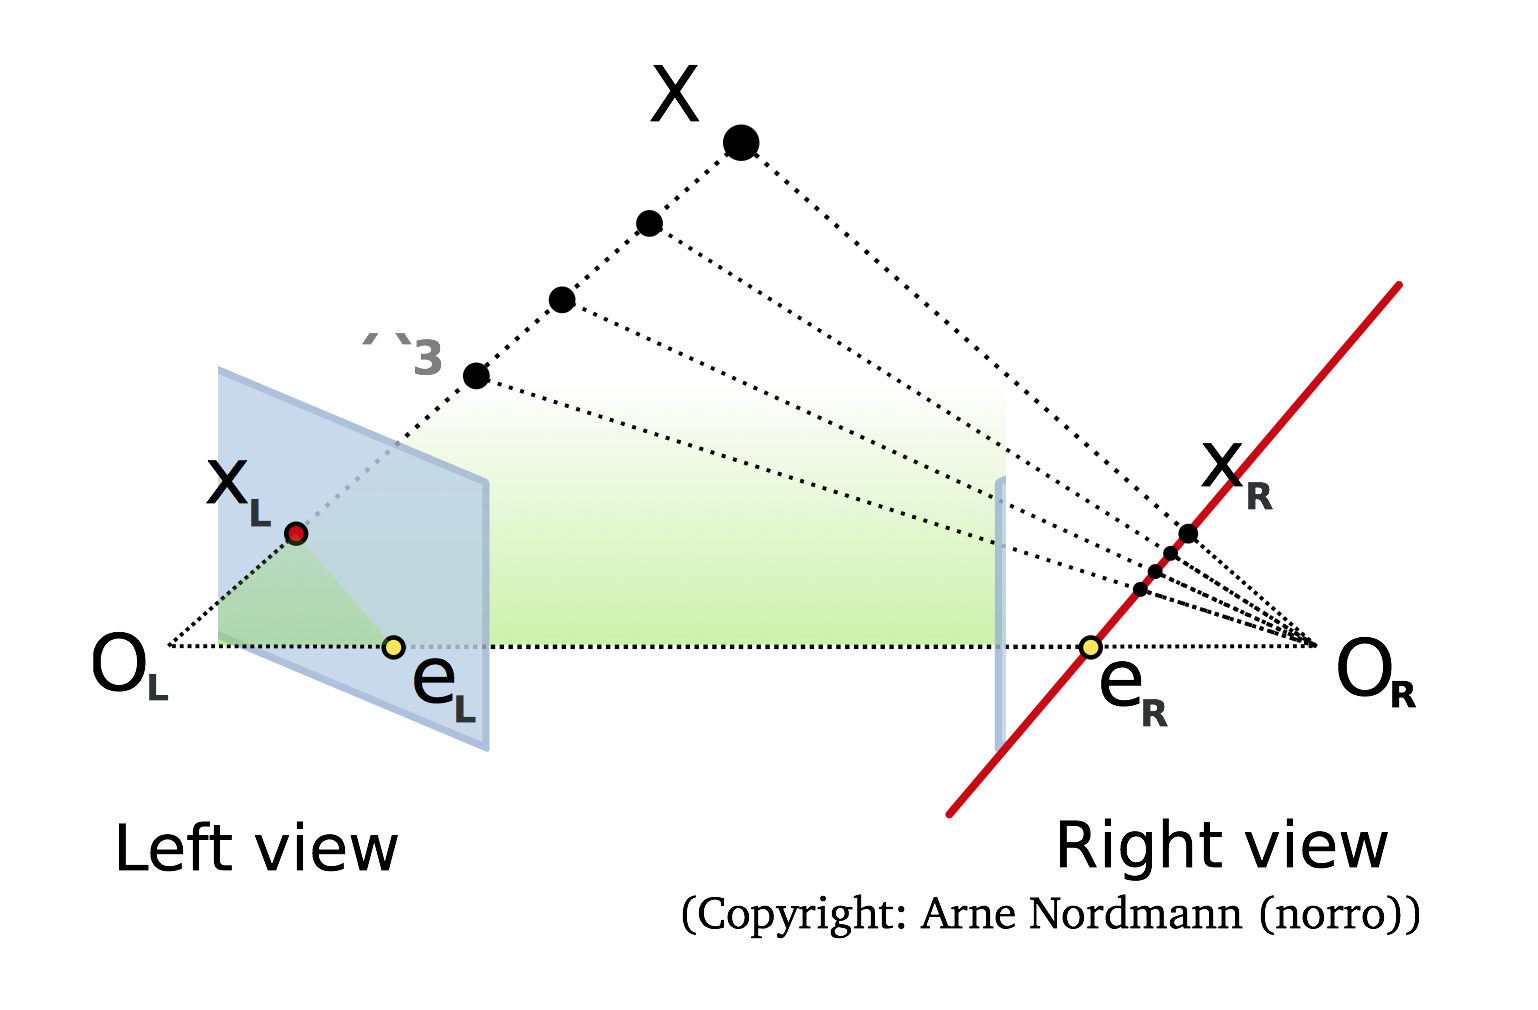
\includegraphics[width=0.4\textwidth]{epipolar_geometry.png}
    \caption{Epipolar geometry.}
    \label{fig:epipolar-geometry}
\end{figure}

\textbf{Epipoles (or epipolar points)}: projection of the focal point of one camera onto the other camera’s image plane (eL and eR)

\textbf{Epipolar plane}: plane defined by the line defined by the focal point and pixel from the source image (OL, XL) focal point of the other camera (OR)

\textbf{Epipolar line}: intersection between the epipolar plane and the image plane of the other camera

Finding the epipolar line is a geometric problem. Simple to solve if images are in the same plane. Alignment of planes may be simulated.

Heuristics for matching:
\begin{compactitem}
    \item Epipolar line (Always valid)
    \item Uniqueness (Always valid)
    \item Ordering (Sometimes valid)
    \item Minimum/maximum disparity (Sometimes valid)
    \item Local continuity (smoothness) (Sometimes valid)
\end{compactitem}

Additional viewpoints leads to more epipolar constraints and more confident matches. But this also leads to issues with the baseline. Dense vs. Sparse matching:
\begin{compactitem}
\item Dense: every pixel has a matching pixel
\item Sparse: only some pixels have a matching pixel. Can concentrate on important, reliable features. Possibility for interpolation.
\end{compactitem}

The depth estimation of a point is given by the equation below. The accuracy of this measure is affected by image noise, and the error in the disparity measure. A longer baseline leads to increased disparity. This leads to a smaller error and better accuracy.
\begin{equation}
    d = \frac{Bf}{x-x'}
\end{equation}
Where $B$ is the baseline, $f$ is the focal point distance, $x$ and $x'$ are points on different image planes and $d$ is the depth estimation. This measure gives a trade of between the baseline size used:

\begin{figure}[H]
    \centering
    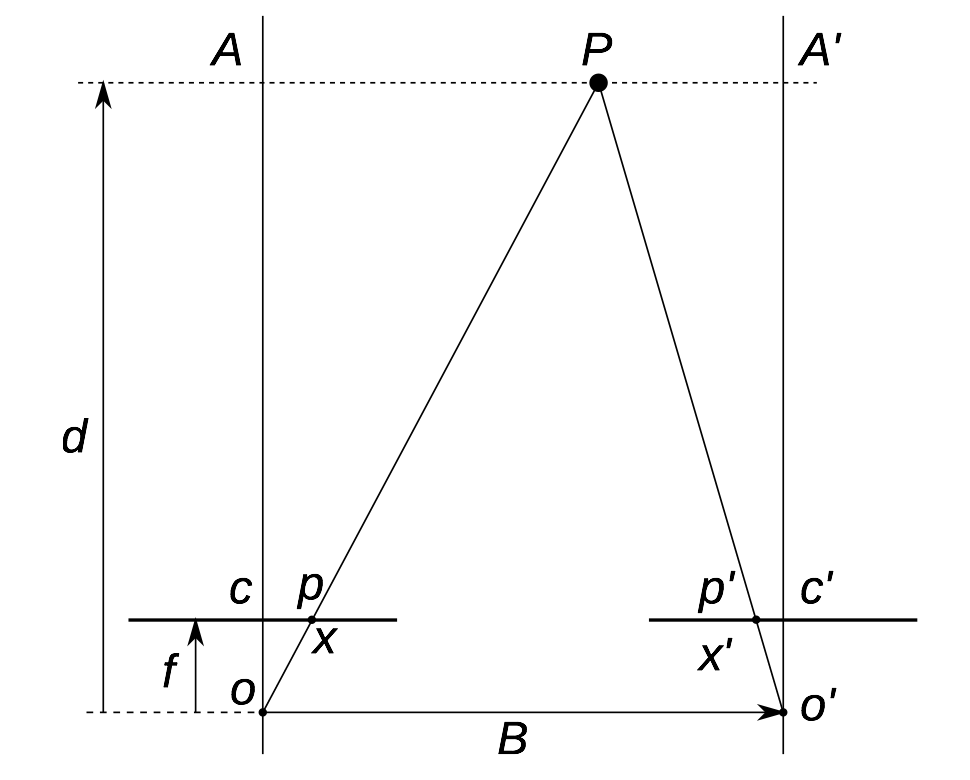
\includegraphics[width=0.4\textwidth]{stereo.png}
    \caption{Epipolar geometry.}
    \label{fig:Stereo depth.}
\end{figure}


\begin{compactitem}
    \item Short baseline: easier matching, fewer occlusions, worse accuracy
    \item Long baseline: difficult matching, more occlusions, better accuracy
\end{compactitem}

\subsection{Calibration Issues}
A.k.a resectioning. Deals with transforming a real camera into a perfect pinhole camera. This is to find the geometry of the camera system.

\textbf{Intrinsic} Parameters of known lens details and effects. Parameters are computed for the focal length, image format, principal point (all using a liner transformation), and lens distortion (using a non-linear transform).

\textbf{Extrinsic} Parameters of known distance between cameras. Parameters are computed to represent translation and rotation between cameras.

In the general case we must find the \textbf{fundermental matrix} that transforms one view to another. This encodes the general geometry of the camera system. You can solve the fundamental matrix given that you have enough matching points between images. As there is noise we usually go for lots of matching points (chessboard texture).

Key points about Stereo:
\begin{compactitem}
    \item Works with a calibrated stereo rig Gives an estimate of depth
    \item Sparse: at features Dense: at every pixel
    \item  Works fairly well, can work real time
\end{compactitem}

\subsection{Structure From Motion}
Moving the cameras give us new problems. We no longer know the baseline, but the camera parameters still only need to be solved once.

Using one camera we can calibrate, take and image, then move it a little bit and take another image. This leads to a constrained search. Issues: Assumption that the camera is only moved a small amount, fundamentally an offline process.

Using Bundler we can use just matched points alone to try and adjust our estimates of 3D surfaces until they fit. The basic process is to get a bunch of images, find out about eh camera (EXIF data), find features using SIFT, match the features, then use Bundler to adjust. Bundler adjustment is an iterative method. It optimises over camera pose, 3D structure and viewing parameters. To do this it uses estimates of the motion and structure, calculates the reprojection error and tries to minimise this. Issues: Very slow!

Key points about SFM:
\begin{compactitem}
    \item Works with uncalibrated cameras Gives an estimate of 3D structure
    \item Returns a point cloud
    \item Gives sparse structure, can’t work anything like real time
    \item Can be re-coloured with texture: triangulate the point cloud, record texture, reproject
\end{compactitem}

\section{3D Vision}
Why would we want to do 3D vision:
\begin{compactitem}
    \item Avoid (or at least mitigate) the difficulty of binocular vision.
    \item Size (and shape) of an object in a scene can be straightforwardly computed from its 3D coordinates.
    \item Objects can be directly rendered for visualisation
    \item You can tell a lot about the world if you know how far away things are directly
\end{compactitem}

Range sensors are used to measure depth. These may measure depth at a single point, shape/surface profiles, or full surfaces. These fall into two major categories:

\textbf{Laserstripe Techniques}: Uses a very fast spinning mirror and a laser to measure depth. The laser provides a phased based measurement and is reconstructed in software. Good for large distances (such as a field). Lecia HDS: 89 metre range and 3mm resolution.

\textbf{Kinect-style Techniques}: Projects infra-red speckle pattern. Measures inference pattern to determine 3D structure. Gives a distance at each speckle point which can be used to reconstruct 3D. Accuracy depends on distance, but is usually good down to millimetres.

Which to use:
\begin{compactitem}
    \item Kinect: cheap, reasonably accurate in “room sized” areas, captures image at a time, can handle motion
    \item Leica: Expensive, very accurate, works up to field scale, captures stripes, doesn’t work well with moving things
    \item both are egocentric!
\end{compactitem}

Occlusions present a challenge to both techniques. Either the laser light doesn't reach part of the scene (laser occlusion) or the camera does not see the area reached by the laser (sensor occlusion). Quality measures:

\begin{compactitem}
    \item Resolution: Smallest change in depth that sensor can report? Quantization? Spacing of samples?
    \item Accuracy: the degree of conformity of a measured quantity to its actual (true) value. Measurement of what?
    \item Repeatability (precision): the degree to which further measurements show the same result. Do the measurements drift?
    \item Environmental sensitivity: Does temperature or wind speed influence measurements?
    \item Speed: Points per second? Seconds per point? Off-line or true realtime?
\end{compactitem}

\subsection{Representation Of Range Data}
\textbf{xyz form or cloud of points (unstructured)}:  a list of 3D coordinates in a given reference frame. No specific order is required.

\textbf{rij form (structured)}: a matrix of depth values of points along the directions of the xy image axes. The points follow a specific order, given by the xs and ys

to render either you simple triangulate the points.

\subsection{Moving to a Common Image Frame}
Range data is egocentric. You have the distance from a scanner to the point in the world. If you want to get a model of the world (and the world is complex) you need to do multiple scans and join them together. This is called registration. The easiest way it to put markers in the scene. Given two overlapping scenes we need to estimate the underlying transformation that brings one image into the best possible alignment with another.

\textbf{Rigid Transformation}: the distance between any two points on the surface will not change before and after the transformation. Consists of rigid rotation matrix and a translation vector. Issues: fine if object is rigid. Assume views are not far apart. Assume there are not major occlusions.

Iterative closest point algorithm:
\begin{enumerate}
    \item Estimate transformation parameters (guess)
    \item Establish tentative point correspondences
    \item Evaluate tentative point correspondences
    \item Estimate transformation parameters (again: this is why it’s called iterative)
    \item Is it good enough? If so, complete. If not, go to 2.
\end{enumerate}

Pros of ICP:
\begin{compactitem}
    \item ``Easy'' to implement without requiring image segmentation and feature extraction
    \item Doesn’t require calibration markers
    \item Has a closed form solution to the underlying transformation parameters of interest
    \item Computationally acceptable: With k-d tree used to accelerate the closest point search, the computational complexity is $O(n log n)$.
\end{compactitem}

Cons of ICP:
\begin{compactitem}
    \item Requires an initial guess at the underlying transformation parameters
    \item Sensitive to occlusion, appearance and disappearance of points Difficult in estimating quality of tentative correspondences
    \item The algorithm converges to a local minimum, instead of global minimum,
    \item The termination condition is difficult to determine
\end{compactitem}

\textbf{Pointclouds}: convex hull, density meaures, triangulate to get surface
\textbf{Surfaces}: surface area, volumetric measurements

\section{Evaluation Techniques}
How can we be sure we’re not cheating?
\begin{compactitem}
    \item Separation of training and test sets
    \item N-fold validation
    \item Careful design of evaluation scenarios and datasets
\end{compactitem}

How can we compare against other techniques?
\begin{compactitem}
    \item Shared, open datasets
    \item Performance statistics which measure the right thing
\end{compactitem}

Large datasets allow use to build systems which work with input that contains a lot of variation. A dataset on its own is not enough. We also need a ground truth. Some have an experimental protocol, some have a explicit training/testing split.

Where does ground truth come from?
\begin{compactitem}
\item Hand labelled. Often by more than one person
\item Part of the acquisition process e.g. deliberately capture N people walking a known path
\item From a different measurement system e.g. we could evaluate a visual tracking system using a gps
\item Bootstrapped. Using “informal” ground truths, like tags from a social network used to learn a face recogniser
\end{compactitem}

\subsection{Performance Measurement \& Reporting}
We have to decide what we really care about. Often we're not too bothered about the location, but we care about the class. The precision required is also important. We can let some incorrect thins through in a pre-processing step that we can deal with later.

\begin{compactitem}
\item \textbf{True positives} It’s there and we say it’s there
\item \textbf{False positives} It’s not there and we say it’s there
\item \textbf{True negatives} It’s not there, and we don’t say it’s there
\item \textbf{False negatives} It’s there, but we say it isn’t
\end{compactitem}

\subsubsection{Confusion matrices}
Can be used for both detectors and classifiers. Very useful to see where the technique is going wrong and what it gets right.

\begin{figure}[H]
    \centering
    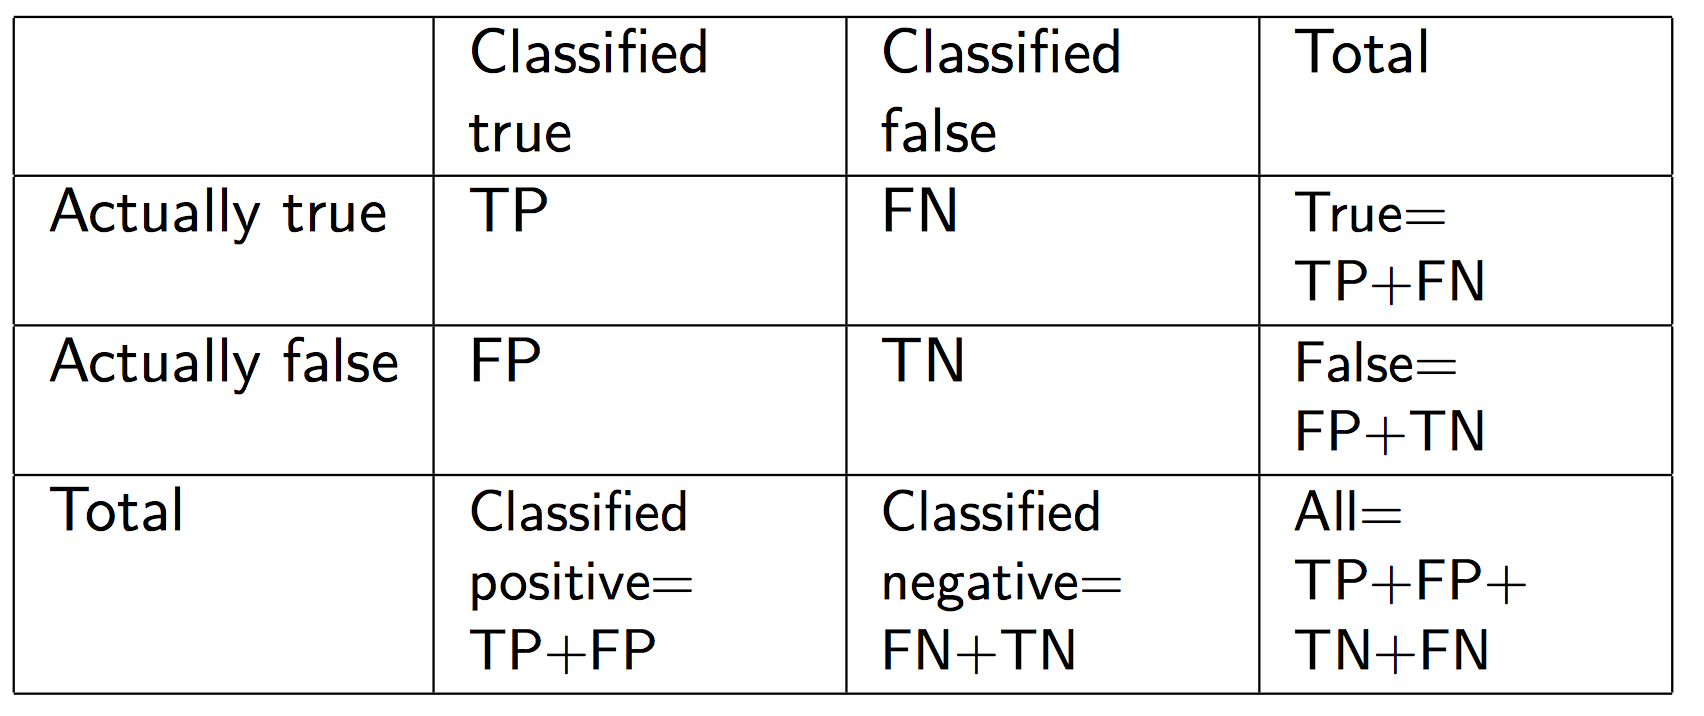
\includegraphics[width=0.4\textwidth]{confusion_matrix.png}
    \caption{Simple confusion matrix.}
    \label{fig:confusion-matrix}
\end{figure}

\begin{figure}[H]
    \centering
    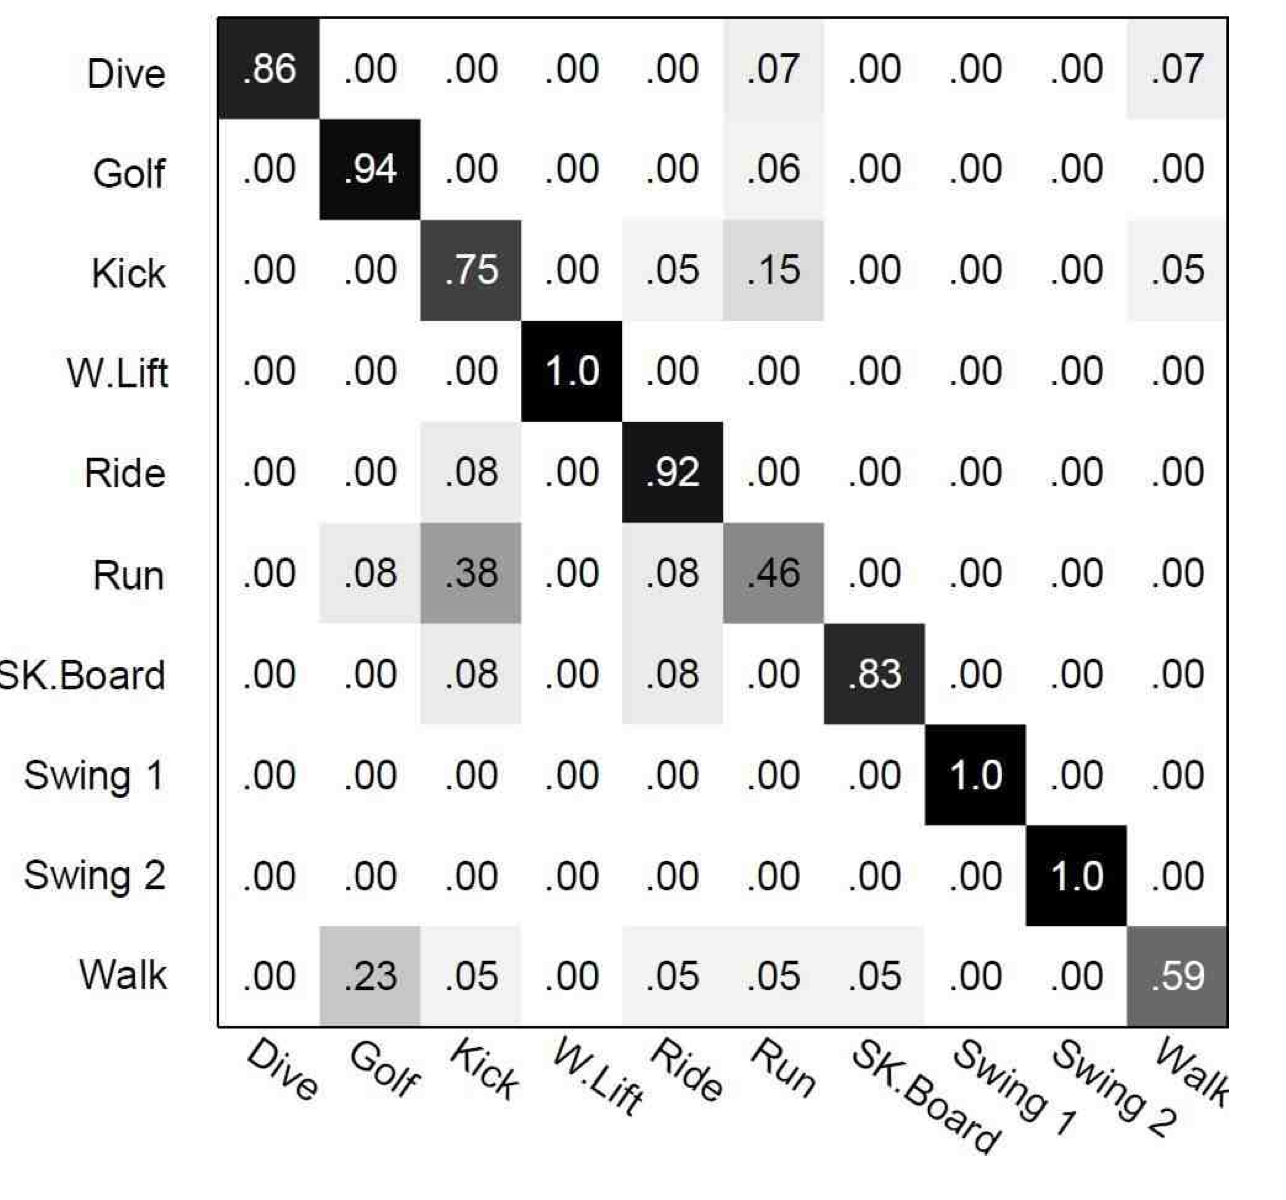
\includegraphics[width=0.3\textwidth]{confusion_matrix_2.png}
    \caption{Multi class confusion matrix.}
    \label{fig:confusion-matrix-2}
\end{figure}

\subsubsection{Reciever Operating Characteristic}
The true positive rate plotted against the false positive rate. Good way to compare different techniques. Excellent way to check performance of a yes/no classifier. Can see the performance of the system as a whole, not just the best performing bit. The area under the curve gives the probability that the classifer will rank a randomly chosen positive example higher than a randomly chosen negative one.

\begin{figure}[H]
    \centering
    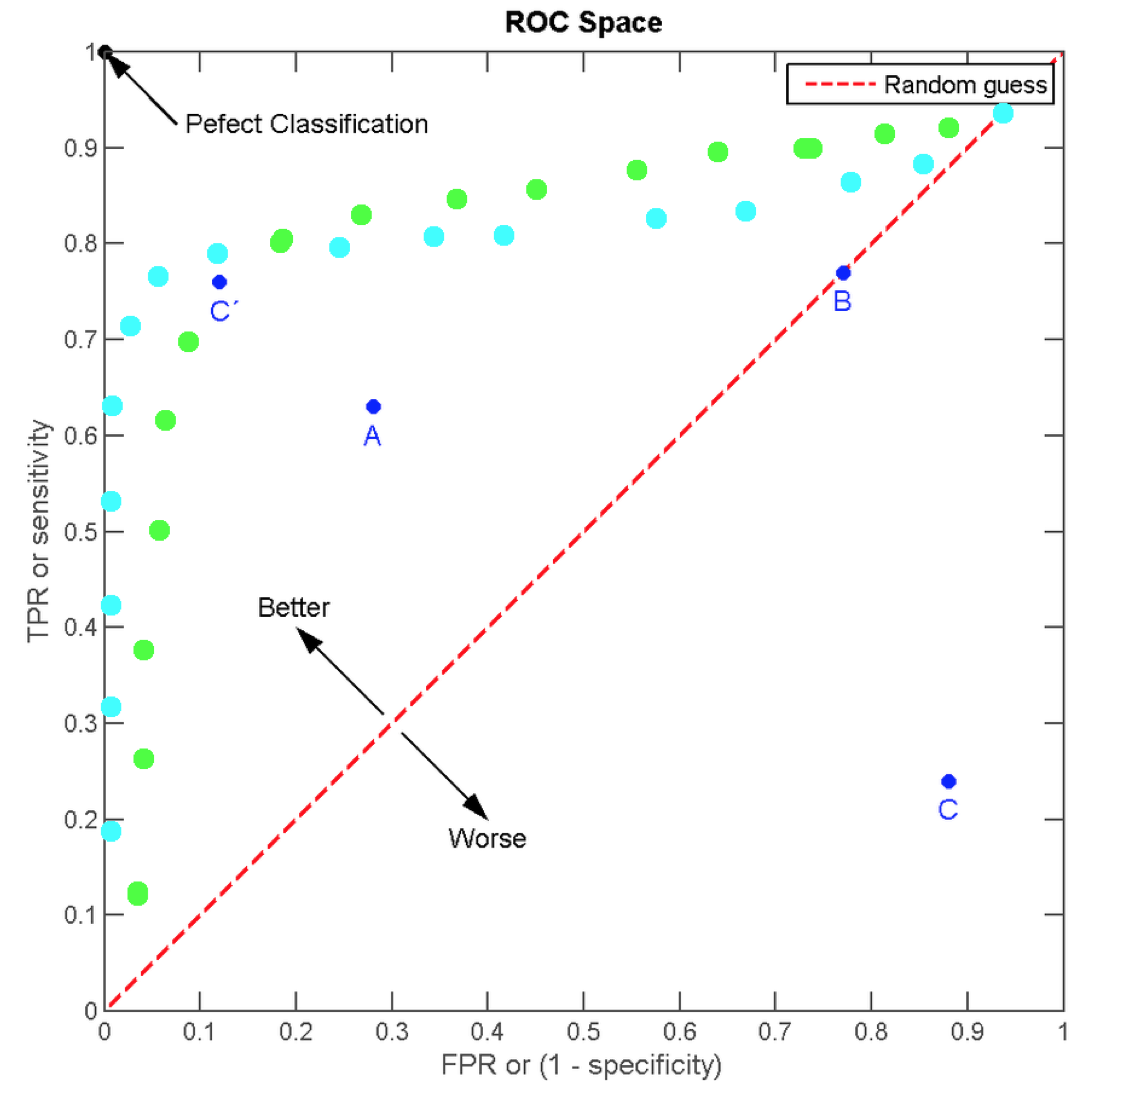
\includegraphics[width=0.3\textwidth]{roc_curve.png}
    \caption{ROC Curve.}
    \label{fig:roc-curve}
\end{figure}

\subsubsection{Distance Measures}
\textbf{Point and Lines}: usually use mean squared error. $\frac{1}{n}\sum(Y - Y')^2$. Mesaures the absolute distance over a set of points. For lines and sets of points sometimes the ordering matters. Sometimes how we match points matters.

\textbf{Areas}: Use bounding box overlap or bounding box union.

\begin{figure}[H]
    \centering
    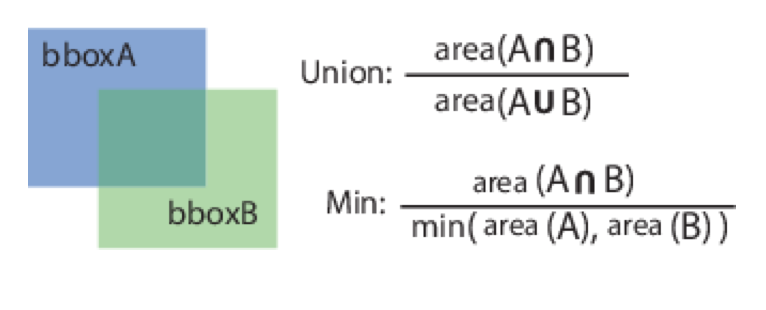
\includegraphics[width=0.3\textwidth]{bounding_box.png}
    \caption{Bounding Boxes.}
    \label{fig:bounding-box}
\end{figure}

\section{Application of method}
What components are required for counting people in a scene?
\begin{compactitem}
    \item One of the most obvious requirements is that it needs to be accurate. How accurate is ``good enough'' is dependant on the system implementation.
    \item Robustness to variance.
    \item Robustness to occlusions.
\end{compactitem}
Questions for consideration.
\begin{compactitem}
    \item Does it need to run at real time?
    \item What's the specific scenario?
    \item How reliable should the count be?
    \item All people or just some?
\end{compactitem}
Key issues with people counting?
\begin{compactitem}
    \item Images of people (whole bodies) have a high degree of variance. Not very many invariant features.
    \item Occlusions a likely to be a problem (Both by objects in the scene and by other people, also hats, caps, shopping bags).
    \item Orientation and rotation of people will be a problem, (side views, people in the opposite direction).
    \item Camera perspective. People further away will have fewer points of interest/smaller resolution.
\end{compactitem}

Counting people in a scene essentially boils down to a classification/detection problem. Given a region of an image can we tell if there is a person in it or not. Then we count the number of successful detections. Potential approaches to solving the problem:

\begin{compactitem}
    \item \textbf{Detection based}: Find the person in the scene. Viola-Jones is an example. Individually detect each individual and therefore count the number of people. \cite{viola2004robust}
    \item \textbf{Indirect}: Density estimation techniques. Measure some features that do not require the separate detection of individual person. Find clusters of interesting features and estimate the density of the clusters. \cite{conte2010method}
\end{compactitem}

Key datasets for people counting:
\begin{compactitem}
    \item PETS - Performance Evaluation of Tracking and Surveillance dataset.
    \item Caltech Pedestrian Detection Benchmark
\end{compactitem}

\bibliographystyle{chicago}
\bibliography{vision.bib}
\end{multicols}
\end{document}
